\section*{Exercises}

\begin{ex}
  Find the matrix for the linear transformation that
  rotates every vector in $\R^2$ by an angle of $\pi /3$.
  \begin{sol}
    $\begin{mymatrix}{cc}
      \cos \paren{
        \frac{\pi }{3}} & -\sin \paren{\frac{\pi }{3}} \\
      \sin \paren{\frac{\pi }{3}} & \cos \paren{\frac{\pi }{3}}%
    \end{mymatrix} = \begin{mymatrix}{cc}
      \frac{1}{2} & -\frac{1}{2}\sqrt{3} \\
      \frac{1}{2}\sqrt{3} & \frac{1}{2}
    \end{mymatrix} $
  \end{sol}
\end{ex}

\begin{ex}
  Find the matrix for the linear transformation that reflects every
  vector in $\R^2$ about the $x$-axis.
\end{ex}

\begin{ex}
  Find the matrix for the linear transformation that reflects every
  vector in $\R^2$ about the line $y=-x$.
\end{ex}

\begin{ex}
  Find the matrix for the linear transformation that stretches $\R^2$
  by a factor of $3$ in the vertical direction.
\end{ex}

\begin{ex}
  Find the matrix of the linear transformation that reflects every
  vector in $\R^3$ about the $xy$-plane.
\end{ex}

\begin{ex}
  Find the matrix of the linear transformation that reflects every
  vector in $\R^3$ about plane $x=z$.
\end{ex}

\begin{ex}
  Describe the linear transformation that is given by each of the
  following matrices. Draw a before-and-after picture for each.
  \begin{equation*}
    (a)\quad
    A = \begin{mymatrix}{rr}
      1 & -1 \\
      1 &  1 \\
    \end{mymatrix},\quad
    (b)\quad
    B = \begin{mymatrix}{rr}
      0 & 2 \\
      1 & 0 \\
    \end{mymatrix},\quad
    (c)\quad
    C = \begin{mymatrix}{rr}
      1 & 0 \\
      -1 & 1 \\
    \end{mymatrix},\quad
    (d)\quad
    D = \begin{mymatrix}{rr}
      1 & 0 \\
      0 & 0 \\
    \end{mymatrix}.
  \end{equation*}
\end{ex}

\begin{ex}
  Let $\vect{u}=\begin{mymatrix}{r} a \\ b \end{mymatrix} $ be a unit
  vector in $\R^2$. Find the matrix%
  \index{reflection!about a given vector} that reflects all vectors
  about this vector, as shown in the following picture.
  \begin{center}
    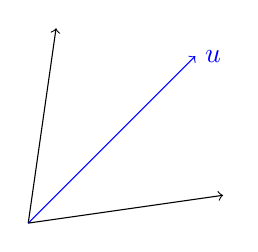
\begin{tikzpicture}[rotate=45]
      \draw[->](0,0)--(2,1.5);
      \draw[blue, ->](0,0) -- (3,0) node [right] {$\vect{u}$};
      \draw[->](0,0)--(2,-1.5);
    \end{tikzpicture}
  \end{center}
  \begin{sol}
    First, we compute $\vect{v}'$, the projection of $\vect{v}$ onto
    $\vect{u}$.
    \begin{center}
      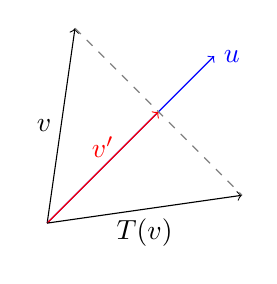
\begin{tikzpicture}[rotate=45]
        \draw[->](0,0) -- node[left] {$\vect{v}$} (2,1.5);
        \draw[blue, ->](0,0) -- (3,0) node [right] {$\vect{u}$};
        \draw[red, ->](0,0) --  node [above] {$\vect{v}'$} (2,0);
        \draw[->](0,0) -- node[below] {$T(\vect{v})$} (2,-1.5);
        \draw[dashed,gray] (2,1.5) -- (2,-1.5);
      \end{tikzpicture}
    \end{center}
    We have
    \begin{equation*}
      \vect{v}'
      = \proj_{\vect{u}} \vect{v}
      = \frac{\vect{u}\dotprod\vect{v}}{\norm{\vect{u}}^2}\,\vect{u}.
    \end{equation*}
    But since $\vect{u}$ is a unit vector, this simplifies to
    $\vect{v}' = (\vect{u}\dotprod\vect{v})\vect{u}$.
    From the above picture, we see that $T(\vect{v}) = \vect{v} +
    2(\vect{v}'-\vect{v}) = 2\vect{v}' - \vect{v} =
    2(\vect{u}\dotprod\vect{v})\vect{u} - \vect{v}$.
    To get the matrix of this linear transformation, we must compute
    the image of the standard basis vectors:
    \begin{equation*}
      T(\vect{e}_1) = 2(\vect{u}\dotprod\vect{e}_1)\vect{u} - \vect{e}_1
      = 2a\begin{mymatrix}{c} a\\b \end{mymatrix} - \begin{mymatrix}{c} 1\\0 \end{mymatrix}
      = \begin{mymatrix}{c} 2a^2-1\\2ab \end{mymatrix}
    \end{equation*}
    \begin{equation*}
      T(\vect{e}_2) = 2(\vect{u}\dotprod\vect{e}_2)\vect{u} - \vect{e}_2
      = 2b\begin{mymatrix}{c} a\\b \end{mymatrix} - \begin{mymatrix}{c} 0\\1 \end{mymatrix}
      = \begin{mymatrix}{c} 2ab\\2b^2-1 \end{mymatrix}.
    \end{equation*}
    Therefore, the matrix is
    \begin{equation*}
      A = \begin{mymatrix}{cc}
        2a^2-1 & 2ab \\
        2ab & 2b^2-1 \\
      \end{mymatrix}.
    \end{equation*}
  \end{sol}
\end{ex}

